% !TeX root = ../Thesis.tex

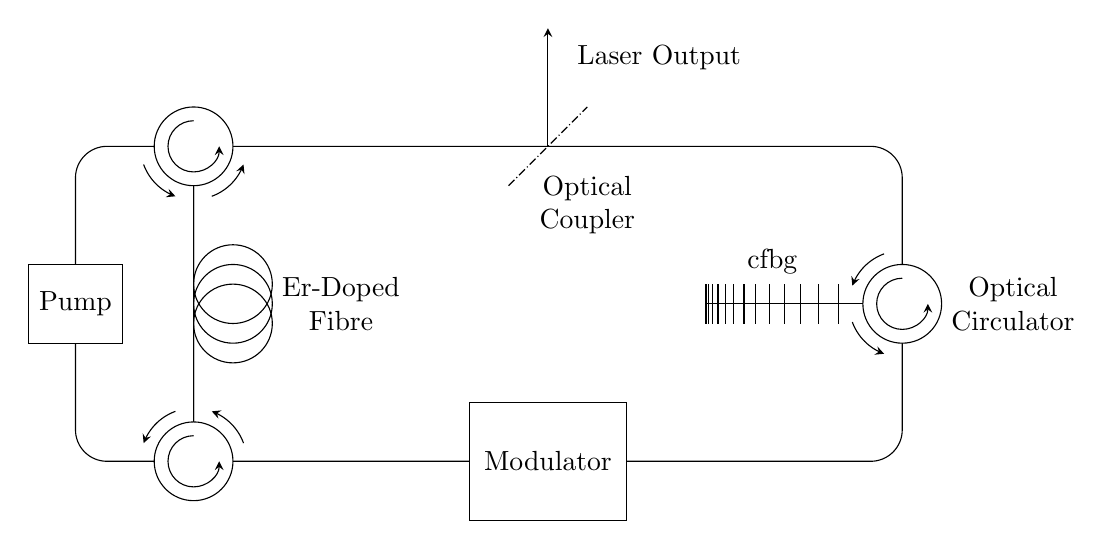
\begin{tikzpicture}
% Two laser loops
\draw [rounded corners=4mm] (0,0) rectangle ++(9,4);
\draw [rounded corners=4mm] (0,0) rectangle ++(-1.5,4);

% Gain
\draw (0.5,2.25) circle (0.5cm);
\draw (0.5,2) circle (0.5cm) node [anchor=west,xshift=0.5cm,align=center] {Er-Doped \\ Fibre};
\draw (0.5,1.75) circle (0.5cm);

% Modulator and pump
\filldraw[fill=white, draw=black] (3.5,-0.75) rectangle ++(2,1.5) node [midway] {Modulator};
\filldraw[fill=white, draw=black] (-2.1,1.5) rectangle ++(1.2,1) node [midway] {Pump};

% Coupler and output
\draw[-stealth] (4.5,4) -- (4.5,5.5) node [pos=0.75,anchor=west,xshift=0.25cm] {Laser Output};
\draw[densely dashdotted] (4,3.5) -- (5,4.5) node [pos=1,anchor=north,yshift=-0.75cm,align=center] {Optical \\ Coupler};

% Circulators
\filldraw[fill=white, draw=black] (9,2) circle (0.5cm) node [anchor=west,xshift=0.5cm,align=center] {Optical \\ Circulator};
\draw[->,>=stealth] (9,2.325) arc (90:360:0.325cm);

\filldraw[fill=white, draw=black] (0,0) circle (0.5cm);
\draw[->,>=stealth] (0,0.325) arc (90:360:0.325cm);

\filldraw[fill=white, draw=black] (0,4) circle (0.5cm);
\draw[->,>=stealth] (0,4.325) arc (90:360:0.325cm);

% Arrows
\draw [->,>=stealth,domain=20:70] plot ({0.675*cos(\x)}, {0.675*sin(\x)});
\draw [->,>=stealth,domain=110:160] plot ({0.675*cos(\x)}, {0.675*sin(\x)});
\draw [->,>=stealth,domain=110:160] plot ({9+0.675*cos(\x)}, {2+0.675*sin(\x)});
\draw [->,>=stealth,domain=200:250] plot ({9+0.675*cos(\x)}, {2+0.675*sin(\x)});
\draw [->,>=stealth,domain=200:250] plot ({0.675*cos(\x)}, {4+0.675*sin(\x)});
\draw [->,>=stealth,domain=290:340] plot ({0.675*cos(\x)}, {4+0.675*sin(\x)});

% Grating
\draw (8.5,2) -- (6.5,2) node [pos=0.5,anchor=south,yshift=0.25cm,xshift=-0.15cm] {\acrshort{cfbg}};
\foreach \i in {0,...,13}
  \draw (6.5 + \i*\i/100,1.75) -- (6.5 + \i*\i/100,2.25);

% Arrows
%\draw[-stealth] (2.16,0) -- (2.15,0);
%\draw[-stealth] (2.39,4) -- (2.4,4);
%\draw[-stealth] (6.76,0) -- (6.75,0);
%\draw[-stealth] (7.09,4) -- (7.1,4);
%\draw[-stealth] (-0.649,0) -- (-0.65,0);
%\draw[-stealth] (-0.351,4) -- (-0.35,4);
\end{tikzpicture}